\documentclass[%
a4paper,
twoside,
12pt
]{article}

% encoding, font, language
\usepackage[T1]{fontenc}
\usepackage[utf8]{inputenc}
\usepackage{lmodern}
\usepackage[ngerman]{babel}

\usepackage{nicefrac}
\usepackage{textcomp}
\usepackage{setspace}

\usepackage[
%    handwritten,
    nowarnings,
    %myconfig
]
{config/xcookybooky}



\DeclareRobustCommand{\textcelcius}{\ensuremath{^{\circ}\mathrm{C}}}


\setcounter{secnumdepth}{1}
\renewcommand*{\recipesection}[2][]
{%
    \subsection[#1]{#2}
}
\renewcommand{\subsectionmark}[1]
{% no implementation to display the section name instead
}


\usepackage{hyperref}    % must be the last package
\hypersetup{%
    pdfauthor            = {Kathrin Welzel and Marcel Gro{\ss}mann},
    pdftitle             = {Wedding Recipes},
    pdfsubject           = {Recipes},
    pdfkeywords          = {wedding, recipes, cookbook},
    pdfstartview         = {FitV},
    pdfview              = {FitH},
    pdfpagemode          = {UseNone}, % Options; UseNone, UseOutlines
    bookmarksopen        = {true},
    pdfpagetransition    = {Glitter},
    colorlinks           = {true},
    linkcolor            = {black},
    urlcolor             = {blue},
    citecolor            = {black},
    filecolor            = {black},
}

\hbadness=10000	% Ignore underfull boxes

\begin{document}
\title{Kochbuch anl"asslich der Hochzeit}
\author{Kathrin Welzel \& Marcel Gro{\ss}mann}

\begin{titlepage}
		\setstretch{1.5}
	\centering\fontsize{80pt}{80pt}\fontfamily{pbk}\selectfont

	Kochbuch
	
	\huge
	anl"asslich der Hochzeit
	
	von
	
	\fontsize{40pt}{40pt}\selectfont
	Kathrin \& Marcel
	
	\vfill
	\begin{figure}[h]
		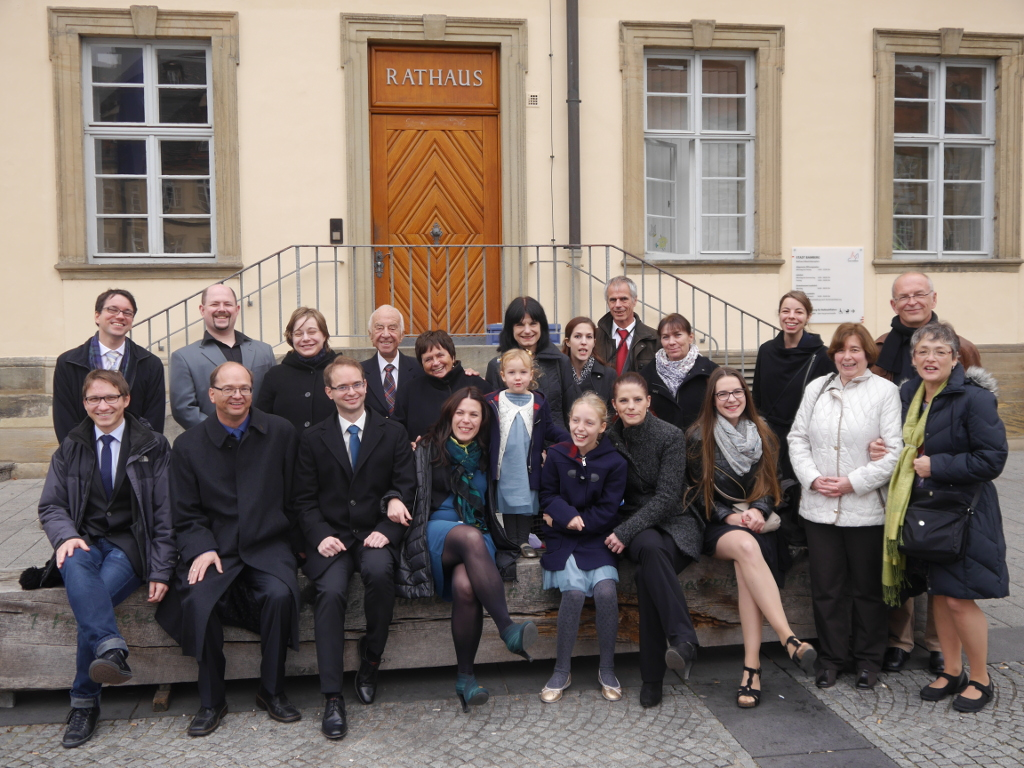
\includegraphics[width=\textwidth]{pic/front.jpg}
	\end{figure}
\LARGE
	\today
\end{titlepage}
\thispagestyle{empty}



\cleardoublepage
\tableofcontents


\cleardoublepage


% background graphic
%\setBackgroundPicture[x, y=-2cm, width=\paperwidth-4cm, height, orientation = pagecenter]{pic/background}

\begin{otherlanguage}{ngerman}
\setHeadlines
{% translation
    inghead = Zutaten,
    prephead = Zubereitung,
    hinthead = Tipp,
    continuationhead = Fortsetzung,
    continuationfoot = Fortsetzung auf n\"achster Seite,
    portionvalue = Personen,
}

%%%%%%%%%%%%%%%%%%%%%%%%%%%%%%%%%%%%%%%%%%%%%%%%%%%%%%%%%%%%%%%%%%%
%				Recipe Section										%
%%%%%%%%%%%%%%%%%%%%%%%%%%%%%%%%%%%%%%%%%%%%%%%%%%%%%%%%%%%%%%%%%%%


\cleardoublepage

\subsection{Herbstrezepte}
\begin{figure}[h]
	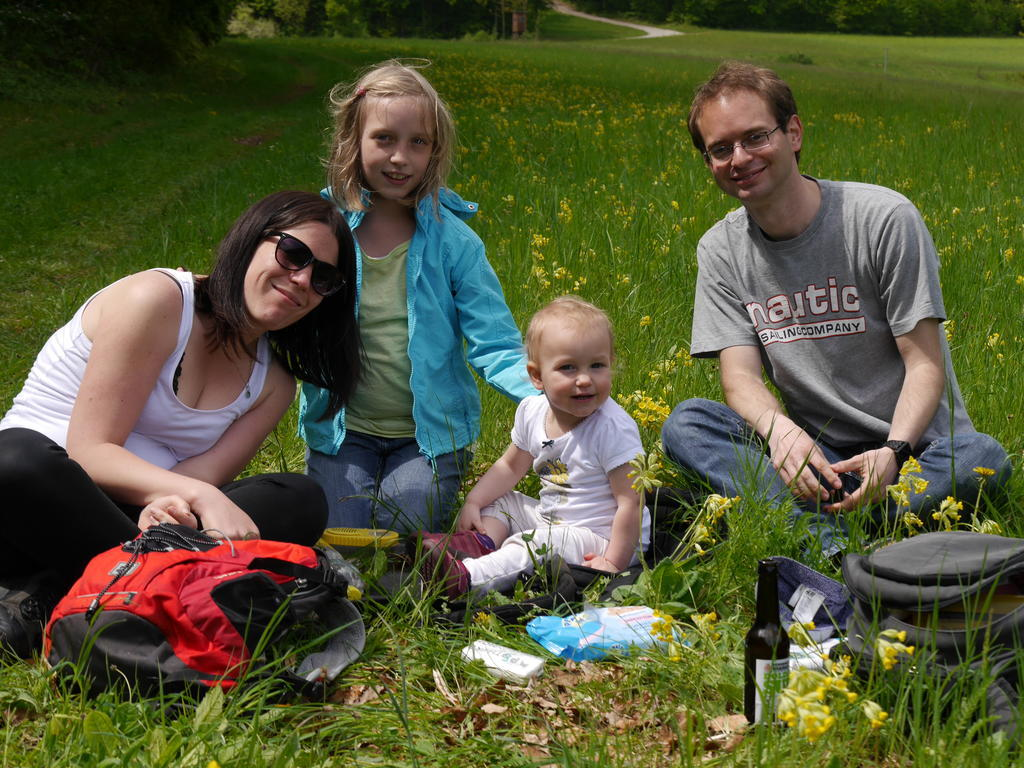
\includegraphics[width=\textwidth]{pic/US}
\end{figure}
\include{recipes/PumpkinSoup}
\include{recipes/CurlyKaleSoup}
\include{recipes/LinsenFenchelEintopf}
\include{recipes/TomatoeBredie}
\include{recipes/BroccoliNoodles}
\include{recipes/MushroomPolenta}
\include{recipes/ColeSlawWok}
\include{recipes/BrokkoliSuesskartoffelAuflauf}
\include{recipes/Cheese}
\include{recipes/AvocadoMouse}


\end{otherlanguage}

\clearpage
~\thispagestyle{empty}
% Last page
\clearpage
\thispagestyle{empty}
~
\vfill
\begin{center}
\begin{tikzpicture}[scale=1.5]
\fill (0,0) -- (-0.2, 0.1) -- (-4, 0) -- (-0.2, -0.1) -- cycle;
\fill (0,0) -- (0.2, 0.1) -- (4, 0) -- (0.2, -0.1) -- cycle;
\fill (0,0) circle (0.1);
\end{tikzpicture}
\end{center}


    Eine hochzeitliche Rezeptesammlung -- Gerichte die wir G"aste lecker finden! Wir hoffen ihr findet die eine oder andere Anregung und denkt beim Kochen und Genießen an uns und das wundersch"one Fest.
    
    Wenn ihr mal ausgeschlafen habt könnt ihr unsere ganzen pull-requests unter \url{https://github.com/whatever4711/cookbook} annehmen.
\end{document} 